\chapter{Entity Trigger Phrases}
This section is adapted from the research paper I co-authored titled ``Entity Triggers: Learning with Explanations for Named Entity Recognition'' which will appear in the 2020 Association for Computational Linguistics conference.



\section{Motivation}
\label{sec:intro}
Recent advances in NER have primarily focused on training neural network models with an abundance of human annotations, yielding state-of-the-art results \cite{LampleNER}. However, NER often requires huge amounts of labeled data (e.g. tens of thousands of labeled sentences). Collecting these human annotations is expensive and time-consuming, especially in technical domains such as biomedical publications, financial documents, legal reports, etc. As we seek to advance NER into more domains with less human effort, how to learn neural models for NER in a annotation-efficient way becomes a crucial research problem.

The standard protocol for obtaining an annotated NER dataset involves an annotator viewing a sentence, selecting token spans as entities, and labeling the spans with their entity types. Because this annotation process provides limited supervision per example, in order to train a high-performance model, it is necessary to collect a large amount of annotations. Given the effort the annotator has already spent analysing the sentence and recognizing the entity, we aim to investigate how we can obtain extra supervision from this entity annotation.

A human's recognition of an unlabeled entity usually depends on cue words or  phrases in the sentence. For instance, we cold infer that the randomized word \underline{Kasdfrcxzv} is likely to be a location entity mention in the sentence ``Tom \textit{traveled} a lot last year \textit{in} \underline{Kasdfrcxzv}.'' We recognize this location entity because of the cue phrase ``\textit{travel} ... \textit{in},'' which indicates that there should be a location entity after the word ``\textit{in}.'' We hypothesize that these cue phrases not only explain the recognition process, but can also help our NER models to learn and generalize faster. We call such entity-associated rational phrases \textit{entity triggers}. Specifically, we define an entity trigger (or trigger for simplicity) as a group of words that can help explain the recognition process of a particular entity in the same sentence. For example, in~\figref{fig:trigex}, \textit{``had ... lunch at''}\footnote{Note that a trigger can be a discontinuous phrase.} and \textit{``where the food''} are two distinct triggers associated with the \textsc{Restaurant} entity ``\underline{Rumble Fish}.'' An entity trigger should be a necessary and sufficient cue for humans to recognize its associated entity even if we mask the entity with a random word. Thus, unnecessary words such as ``fantastic'' should not be  considered part of the entity trigger.

\begin{figure}[h]
	\centering
% 	\hspace*{-.27in}
	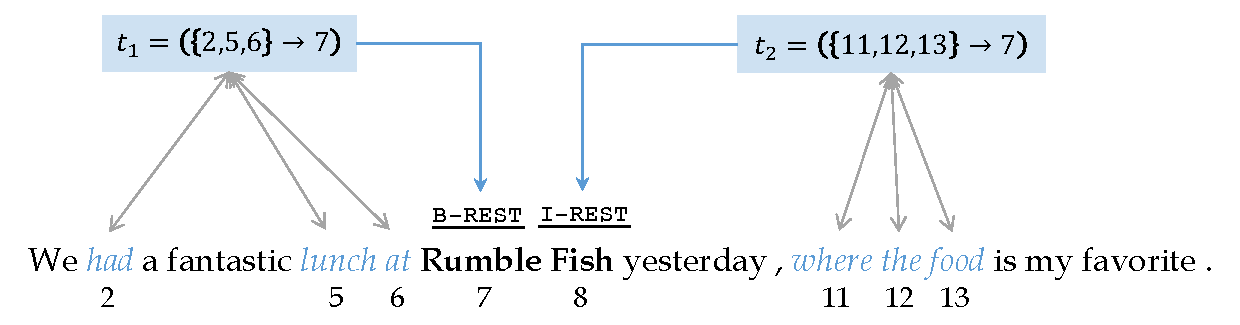
\includegraphics[width=0.85\linewidth]{LatexDiss/figures/trigexample.pdf}
	\caption{Example of entity triggers: \textit{``had(2) ... lunch(5) at(6)''} and \textit{``where(11) the(12) food(13)''} are two individual entity triggers associated to the entity mention {\underline{``Rumble Fish''}} typed as \texttt{REST}aurant, which starts at the 7th token.}
% 	\vspace{-10pt}
	\label{fig:trigex}
\end{figure}

We argue the benefits of supervising models using a combination of entity triggers and standard entity annotations. This approach is more powerful because unlabeled sentences, such as ``Bill \textit{enjoyed} a great \textit{dinner} with Alice \textit{at} \underline{Zcxlbz}.'' can be matched with the existing trigger ``\textit{had} ... \textit{lunch at}'' via their semantic relatedness. This makes it easier for NER models to recognize \underline{Zcxlbz} as a \textsc{Restaurant} entity than if we had only trained the NER model using entity labels. In contrast, if we only had the entity annotation itself (i.e. ``\underline{Rumble Fish}'') as supervision, the model would require many similar examples in order to learn this simple pattern. Annotating triggers in addition to entities is not significantly more laborious since annotators have already read the sentences and analysed the entities. Thus, we hypothesize that using triggers as additional supervision is a more cost-effective way to train models.

We crowd-sourced 14,708 triggers on two well-studied NER datasets to study the usefulness of entity triggers. We proposed a novel framework named \textit{Trigger Matching Network} ({TMN}). Because it exploits triggers, TMN is more powerful and cost-effective than standard approaches. The TMN framework consists of three components: 1) a trigger encoder, 2) a semantic trigger matching module, and 3) an entity tagger. Our first learning stage jointly trains the trigger encoder and semantic trigger matching module. We then learn a sequence tagger using trigger-enhanced attentions in order to incorporate existing trigger information into entity predictions on unseen sentences.

Our contributions are as follows:
\begin{itemize}
    \item We introduced the concept of ``entity triggers,'' a novel form of explanatory annotation for named entity recognition problems.  We crowd-sourced and publicly released 14k annotated entity triggers on two popular datasets: \textit{CoNLL03} (generic domain), \textit{BC5DR} (biomedical domain).
    \item We proposed a novel learning framework, named \textit{Trigger Matching Network}, which encodes entity triggers and softly grounds them on unlabeled sentences to increase the effectiveness of the base entity tagger (Section~\ref{sec:tmn}). 
    \item Experimental results (Section~\ref{sec:exp}) show that the proposed trigger-based framework is significantly more cost-effective. The TMN only uses 20\% of the trigger-annotated sentences from the original CoNLL03 dataset and achieves comparable performance to the conventional model using 70\% of the annotated sentences. 
\end{itemize}





\section{Problem Formulation}
We consider the problem of how to cost-effectively learn a model for NER using entity triggers. This section introduces basic notations and provides a formal task definition for learning using entity triggers.

In the conventional setup for supervised learning for NER, we let $\mathbf{x}=[x^{(1)}, x^{(2)}, \cdots, x^{(n)}]$ denote a sentence in the labeled training corpus $\mathcal{D}_{L}$.
Each labeled sentence has a NER-tag sequence $\textbf{y}=[y^{(1)}, y^{(2)}, \cdots, y^{(n)}]$, where $y^{(i)}\in \mathcal{Y}$ and  $\mathcal{Y}$ can be \{\texttt{O}, \texttt{B-PER}, \texttt{I-PER}, \texttt{B-LOC}, \texttt{I-LOC}, $\cdots$\}. Here, \texttt{O} represents a non-entity, \texttt{B-TYPE} represents the beginning of an entity of type \texttt{TYPE} and \texttt{I-TYPE} remaining words in an entity. The possible tags come from a BIO or BIOES tagging schema for segmenting and typing entity tokens.
Thus, we have $\mathcal{D}_{L}=\{(\mathbf{x_i}, \mathbf{y_i})\}$, and an unlabeled corpus $\mathcal{D}_{U}=\{\mathbf{x_i}\}$ that we want to label.

We use $T(\mathbf{x},\mathbf{y})$ to represent the set of annotated entity triggers, where each trigger $t_i\in T(\mathbf{x},\mathbf{y})$ is associated with an entity index $e$ and a set of word indices $\{w_i\}$.
Note that we use the index of the first word of an entity as its entity index.
That is, $t = (\{w_1, w_2, \cdots\}\rightarrow{e})$, where $e$ and $w_i$ are integers in the range of $[1,|\mathbf{x}|]$. \quad
For instance, in the example shown in Figure~\ref{fig:trigex}, the trigger \textit{``had ... lunch at''} can be represented as a trigger $t_1=(\{2,5,6\}\rightarrow{7})$, because this trigger specifies the entity starting at index $7$, \textit{``Rumble''}, and it contains a set of words with indices: \textit{``had''} ($2$), \textit{``lunch''} ($5$), and \textit{``at''} ($6$).
Similarly, we can represent the second trigger \textit{``where the food''} as $t_2 = (\{11,12,13\}\rightarrow{7})$.
Thus, we have $T(\mathbf{x},\mathbf{y})=\{t_1, t_2\}$ for this sentence.

Adding triggers creates a new form of data $\mathcal{D}_{T} = \{(\mathbf{x_i},\mathbf{y_i}, T(\mathbf{x_i},\mathbf{y_i})\}$. 
Our goal in this paper is to learn a model for NER from a trigger-labeled dataset $\mathcal{D}_T$, such that we can achieve comparable learning performance to a mdoel using a much larger $\mathcal{D}_L$.





\section{Proposed Framework}
\label{sec:tmn}
This section presents our framework for a more cost-effective learning method for NER using triggers. Our intuition is to treat triggers as soft templates such that new sentences can be matched with these triggers via their deep semantic relatedness in inference time. Recall the trigger matching example we discussed in Section~\ref{sec:intro}. By using soft matching via semantic relatedness rather than hard matching via character similarity, we are able to match sentences such as ``Bill \textit{enjoyed} a great \textit{dinner} with Alice \textit{at} \underline{Zcxlbz}.'' to the semantically similar trigger ``\textit{had} ... \textit{lunch at}.''
In order to soft match entity triggers, we need a trainable way to learn trigger representations (i.e. \textit{trigger vectors}).
Given trigger vectors, we can train a model to label each token in the unlabeled sentences with a NER tag using the trigger vectors as extra supervision.
We propose a straightforward yet effective framework, named \textit{Trigger Matching Networks} (TMN), consisting of a trigger encoder ({\texttt{TrigEncoder}}), a semantic-based trigger matching module (\texttt{TrigMatcher}), and a base {sequence tagger} (\texttt{SeqTagger}). 
We have two learning stages for the proposed framework: the first stage (Section~\ref{sec:firststage}) jointly learns the \texttt{TrigEncoder} and \texttt{TrigMatcher}, and the second stage (Section~\ref{sec:secondstage}) uses the trigger vectors to learn NER tag labels.
Figure~\ref{fig:framework} shows this pipeline. We introduce the inference in Section~\ref{sec:inference}.




\subsection{Trigger Encoding and Semantic Trigger Matching}
\label{sec:firststage}
% {\texttt{TrigEncoder}} encodes triggers into entity-aware trigger vectors by learning the mapping between triggers and entity types using simple classification. \texttt{TrigMatcher} is a neural function that matches sentences and triggers by learning the semantic similarity between the two. These two modules are jointly learned so that {\texttt{TrigEncoder}} can embed entity-type knowledge into the trigger vectors and \texttt{TrigMatcher} can embed semantic knowledge into the trigger vectors.

%TODO add red arrow from group to trigger representation
\begin{figure*}[h]  %TODO float figure right here
 	\centering 
% \hspace{-15pt}
	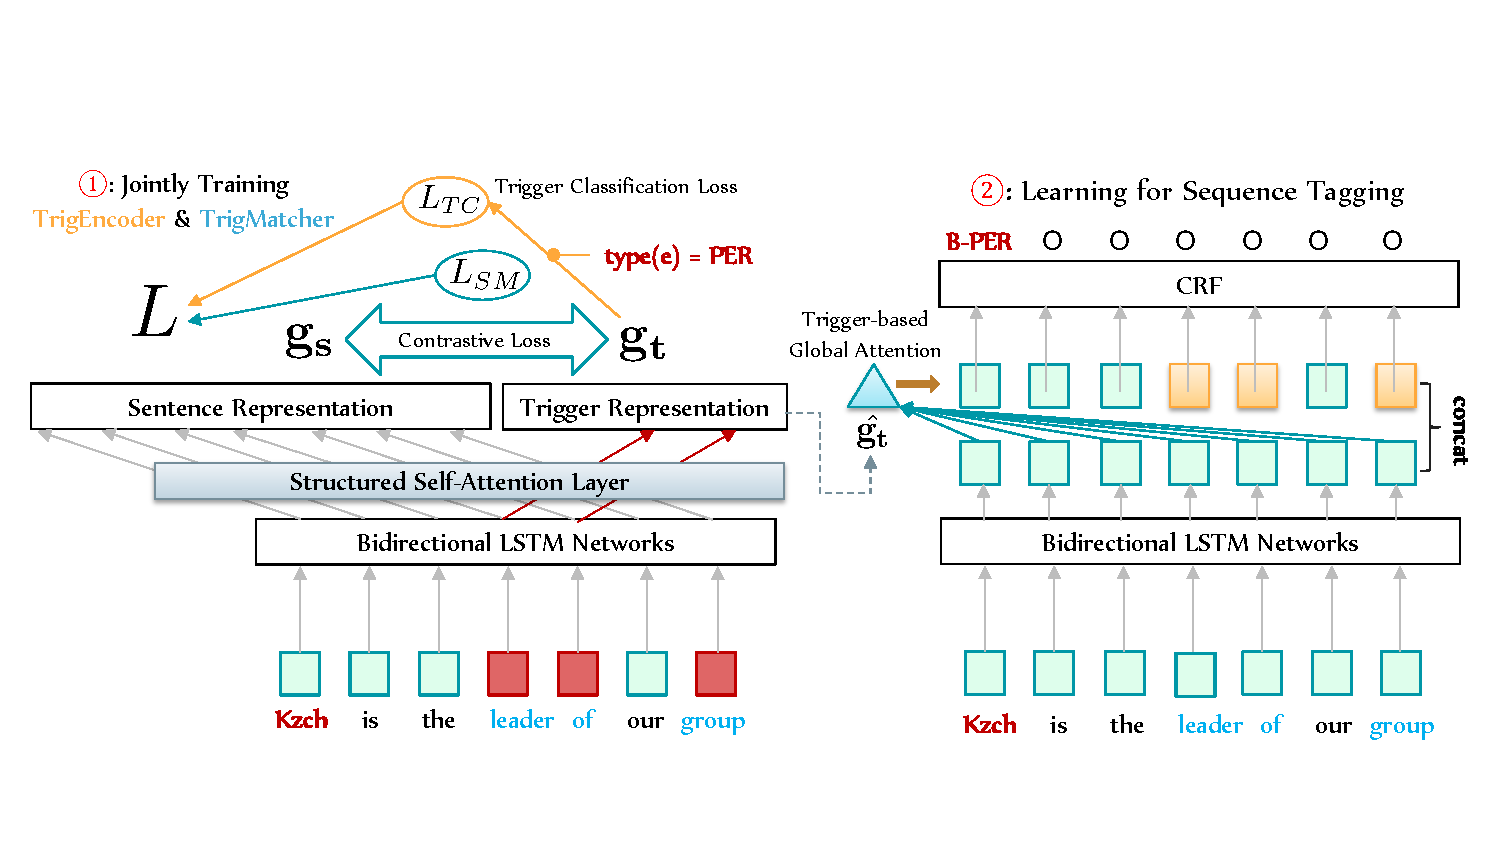
\includegraphics[width=0.85\linewidth]{LatexDiss/figures/tmn.pdf}
	\caption{Two-stage training of the \textit{Trigger Matching Network}. We first jointly train the {\texttt{TrigEncoder}} (via trigger classification) and the \texttt{TrigMatcher} (via contrastive loss). Then, we reuse the training data trigger vectors as attention queries in the \texttt{SeqTagger}.} 
	\label{fig:framework}
\end{figure*}

Learning trigger representations and semantically matching them with sentences are inseparable tasks.
Desired trigger vectors capture the semantics in a shared embedding space with token hidden states such that sentences and triggers can be semantically matched.
Learning an attention-based matching module between entity triggers and sentences is necessary so that triggers and sentences can be semantically matched.
Therefore, as the first learning stage, we propose to jointly train the trigger encoder (\texttt{TrigEncoder}) and the attention-based trigger matching module (\texttt{TrigMatcher}) using a shared embedding space.

Specifically,
for a sentence $\mathbf{x}$ with multiple entities $\{e_1, e_2,\cdots\}$, for each entity $e_i$ we assume that there is a set of triggers $T_i=\{t^{(i)}_1, t^{(i)}_2, \cdots\}$.
To enable more efficient batch-based training, we reform the trigger-based annotated dataset $\mathcal{D}_{T}$ such that each new sequence contains only one entity and one trigger.
We then create a training instance by pairing each entity with one of its triggers, denoted $(\mathbf{x}, e_i, t^{(i)}_j)$.
The learning objective in this stage is to output the tag sequence $\mathbf{y}$. %TODO is this still the learning objective? Isn't the learning objective here the trigger classification loss and contrastive loss?


For each reformed training instance $(\mathbf{x}, e, t)$, we first apply a bidirectional LSTM (BLSTM) 
% TODO  add reference to intro section about BLSTM
on the sequence of word vectors\footnote{Here, by ``word vectors'' we mean the concatenation of external GloVe~\cite{Pennington2014GloveGV} word embeddings and char-level word representations from a trainable CNN network~\cite{DBLP:conf/acl/MaH16}. } 
%TODO read the trainable CNN paper
of $\mathbf{x}$, obtaining a sequence of hidden states that are the contextualized word representations $\mathbf{h}_i$ for each token $x_i$ in the sentence. 
We use $\mathbf{H}$ to denote the matrix containing the hidden vectors of all of the tokens, and we use $\mathbf{Z}$ to denote the matrix containing the hidden vectors of all of the trigger tokens inside the trigger $t$.

In order to learn an attention-based
% TODO add reference to attention  section in intro
representation of both triggers and sentences, we follow the self-attention method introduced by ~\cite{selfattentive} as follows:
{
{ % TODO  add explanation
		\begin{align*} 
			\vec{a}_{sent}&=\operatorname{SoftMax}\left(W_{2} \tanh \left(W_{1} \mathbf{H}^{T}\right)\right)\\
			\mathbf{g_s}&=\vec{a}_{sent}\mathbf{H}\\
			\vec{a}_{trig}&=\operatorname{SoftMax}\left(W_{2} \tanh \left(W_{1} \mathbf{Z}^{T}\right)\right)\\
			\mathbf{g_t}&=\vec{a}_{trig}\mathbf{Z}
		\end{align*} 
	}
}  
$W_1$ and $W_2$ are two trainable parameters for computing self-attention score vectors $\vec{a}_{sent}$ and $\vec{a}_{trig}$, essentially the level of importance the self-attention layer has given to each token.
We obtain a vector representing the weighted sum of the token vectors in the entire sentence as the final sentence vector $\mathbf{g_s}$. Similarly, $\mathbf{g_t}$ is the final trigger vector, representing the weighted sum of the token vectors in the trigger.

We want to use the type of the associated entity as supervision to guide the trigger representation.
Thus, the trigger vector $\mathbf{g_t}$ is further fed into a multi-class classifier to predict the \textit{type} of the associated entity $e$ (such as \texttt{PER}, \texttt{LOC}, etc) which we use $\texttt{type}(e)$ to denote.
The loss of the trigger classification is as follows:
{
	{
		\begin{align*} 
		L_{TC}=-\sum \log \mathrm{P} \left(\texttt{type}(e)~|~ \mathbf{g_t}; \theta_{TC}\right) %  TODO define theta
		\end{align*} 
	}
}  
In order to learn to match triggers and sentences based on their attention-based representations, we use contrastive loss \cite{hadsell2006dimensionality}.
The intuition is that a similar trigger and sentence should have similar representations (i.e. have a small distance betweeen them, $d$).
We randomly mix the triggers and sentences so that we have negative examples (i.e. mismatches) because \texttt{TrigMatcher} needs to be trained with both positive and negative examples of the form (sentence, trigger, label). For the negative examples, we expect a margin $m$ between their representations. The contrastive loss of the soft matching his defined as follows, where $\mathds{1}_{\text{matched}}$ is $1$ if the trigger was originally in this sentence and $0$ if they are mismatched:
{
	{
		\begin{align*}  
		d&=\left\|\mathbf{g_s}-\mathbf{g_t}\right\|_{2}\\
			L_{SM} = (1-\mathds{1}_{\text{matched}}) &\frac{1}{2}\left(d\right)^{2}+\mathds{1}_{\text{matched}} \frac{1}{2}\left\{\max \left(0, m-d\right)\right\}^{2}
		\end{align*} 
	}
}  

Thus, the joint loss we aim to optimize is $L = L_{TC} + \lambda L_{SM}$. % TODO define lambda



\subsection{Trigger-Enhanced Sequence Tagging for NER}
\label{sec:secondstage}
Following the most common design of neural NER architecture, BLSTM-CRF~\cite{DBLP:conf/acl/MaH16}, we incorporate the entity triggers as attention queries 
% TODO cite attention explanation in intro
to train a trigger-enhanced sequence tagger for NER. Note that the BLSTM used in the the \texttt{TrigEncoder} and \texttt{TrigMatcher} modules is the same BLSTM we use in the \texttt{SeqTagger} to obtain $\mathbf{H}$, the matrix containing the hidden vectors of all of the tokens.
Given a sentence $\mathbf{x}$, we use the previously trained \texttt{TrigMatcher} to compute the mean of all the trigger vectors $\hat{\mathbf{g_t}}$ associated with this sentence.
Following the conventional attention method~\cite{luong2015effective}, 
we incorporate the mean trigger vector as the query, creating a sequence of attention-based token representations, $\mathbf{H}'$.
{
    {
        \begin{align*} 
            \vec{\alpha}  &= \operatorname{SoftMax}\left(\boldsymbol{v}^{\top} \tanh \left({U}_{1}\mathbf{H}^T + {U}_{2}\hat{\mathbf{g_t}}^T \right)^{\top}\right)\\
            \mathbf{H'} &=  \vec{\alpha}~\mathbf{H}
        \end{align*} 
    }
}
\noindent
where $U_1$, $U_2$, and $v$ are trainable parameters for computing the trigger-enhanced attention scores for each token.
Finally, we concatenate the original token representation $\mathbf{H}$ with the trigger-enhanced one $\mathbf{H}'$ as the input ($[\mathbf{H};\mathbf{H}']$) to the final CRF tagger.
Note that in this stage, our learning objective is the same as conventional NER, which is to correctly predict the tag for each token.




\subsection{Inference on Unlabeled Sentences}
\label{sec:inference}

When inferencing tags on unlabeled sentences,
we do not know the sentence's triggers.
Instead, we use the \texttt{TrigMatcher} to compute the similarities between the self-attended sentence representations and the trigger representations, using the most suitable triggers as additional inputs to the \texttt{SeqTagger}.
Specifically, we have a trigger dictionary from our training data, $\mathcal{T}=\{t | (\cdot, \cdot, t) \in \mathcal{D}_T\}$.
Recall that we have learned a trigger vector for each of them, and we can load these trigger vectors as a look-up table in memory.
For each unlabeled sentence $\mathbf{x}$, we first compute its self-attended vector $\mathbf{g_s}$ as we do when training the \texttt{TrigMatcher}.
Using L2-norm distances to compute the contrastive loss, we efficiently retrieve the most similar triggers in the shared embedding space of the sentence and trigger vectors.
Then, we calculate $\hat{\mathbf{g_t}}$, the mean of the top $k$ nearest semantically matched triggers, and use it as the attention query for \texttt{SeqTagger}, as we did in Section~\ref{sec:secondstage}.
Now, we can produce trigger-enhanced sequence predictions on unlabeled sentences, as shown in \figref{fig:inference}.

\begin{figure*}[h]
 	\centering 
% \hspace{-15pt}
	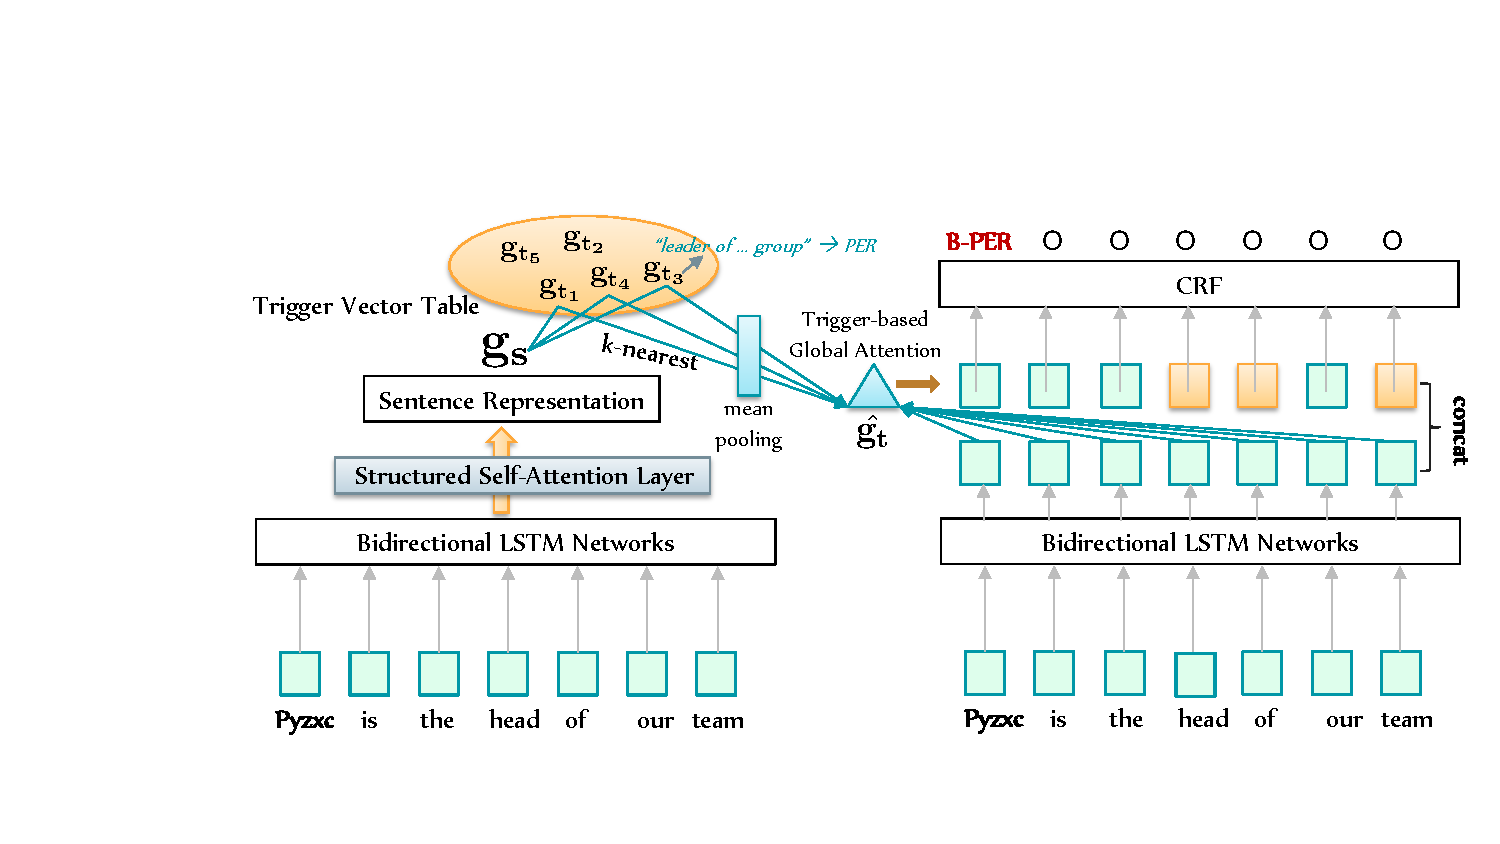
\includegraphics[width=0.85\linewidth]{LatexDiss/figures/inference.pdf}
	\caption{The \textit{inference} process of the TMN framework. It uses the \texttt{TrigMatcher} to retrieve the k nearest triggers and average their trigger vectors as the attention query for the previously trained \texttt{SeqTagger}. This is how a previously unseen cue phrase (e.g., \textit{``head of ... team''}) can be matched with a previously seen trigger (e.g., \textit{``leader of ... group''}).} 
	\label{fig:inference}
\end{figure*}

\section{Experiments}
\label{sec:exp}

\section{Conclusion}